\section{Program Structure and Execution}
    \subsection{Information Storage}
    Computers store information as a series of bits. These bits can be interpreted by users in either source binary, comfortable decimal, or compatible hexadecimal.

    Computers also have a default word size, i.e.\ the largest continuous block of memory the computer can access. Currently, most computers are 32 bit, however more are becoming 64.

    Going with word size, each data type also has a typical size in memory:

    \begin{table}[ht]
        \centering
        \begin{tabular}{l l l}
            {\ttfamily C} Declaration & 32 Bit & 64 Bit\\
            \hline
            char & 1 & 1\\
            short int & 2 & 2\\
            int & 4 & 4\\
            long int & 4 & 8\\
            long long int & 8 & 8\\
            char* & 4 & 8\\
            float & 4 & 4\\
            double & 8 & 8\\
        \end{tabular}
        \label{table:datatypesizes}
        \caption{Size of {\ttfamily C} Data Types}
    \end{table}

    Besides the bits themselves, the order also matters, which brings up the distinction between little-endian and big-endian\footnote{Name arises from Gulliver's Travels}. Big Endian has the highest place values put in the lowest memory location, while Little Endian has the lowest place values put in the lowest memory location.

    \subsection{Integer Arithmetic}
    Depending on the type of numbers involved in addition, we can get strange or unexpected behavior.

    If we're dealing with large numbers, ones that are near to the word size in length, we have to be concerned about overflow. Overflow occurs when the full integer result cannot fit within the word size limits of the given data type.

    Unsigned integer addition results in a something that resembles modular addition. If we have signed integers, we need to now concern ourselves with the negative numbers as well. Negative overflow often results in a positive number due to the definition of two's complement.\footnote{Computers express negative numbers by essentially inverting the bits. Normal binary adds each place, this version subtracts each place from the highest set bit. For a 4 bit word size, the number 1011 would actually be -5 instead of 11.}

    \subsection{Floating Point}
    The first method of expressing floating point numbers for a computer was through fractional binary numbers. These numbers had the form:
    \[ \overbrace{b_m}^{2^m} \overbrace{b_{m-1} }^{2^{m-1} } \cdots \overbrace{b_1}^{2} \overbrace{b_0}^{1} . \underbrace{b_{-1} }_{1/2} \underbrace{b_{-2} }_{1/4} \cdots \underbrace{b_{-n-1} }_{1/2^{n-1} } \underbrace{b_{-n} }_{1/2^n} \]

    The inherent issue with this method, is that it's not very good at dealing with larger numbers. This is where IEEE floating point standard comes in, which has the form:
        \[
            V = (-1)^s \times M \times 2^E
        \]
    Where:
        \begin{easylist}[itemize]
            & $s$ determines sign
            & $M$ is a fractional binary number ranging from $1$ and $2 - \epsilon$ or between $0$ and $1-\epsilon$
            & $E$ weighs the number by a power of 2.
            & Final format looks as such:
                \[ \boxed{S}\boxed{E}\boxed{M} \]
        \end{easylist}

    With these floating point numbers, we have three cases to deal with.

        \begin{easylist}[enumerate]
            & \textbf{Normalized Values} are the most common. This occurs when $E$ is neither all ones nor all zeros.
            & \textbf{Denormalized Values} occur when the exponent field is all zeros. These values express zero, as well as numbers that are very close to zero in absolute value.
            & \textbf{Special Values} occur when the exponent field is all ones. This either indicates $\pm \infty$ or {\ttfamily NaN} when the fractional value is non-zero.
        \end{easylist}

\section{Machine Level Representation of Programs}
Most computers primarily use assembly for a more human-readable machine code. This code is much more explicit than the {\ttfamily C} that it was derived from.

Several fields that are visible in assembly that we lacked access to before:\footnote{For sake of simplicity, all memory addresses are for 32 bit platforms only.}
    \begin{easylist}[itemize]
        & The program counter, referred to as PC, and called {\ttfamily \%eip}, refers to the address in memory of the next instruction to be executed.
        & The integer register file contains eight named locations storing 32 bit values.
        & Condition code registers
        & Floating point registers
    \end{easylist}

    There are a number of different commands that assembly uses in order to provide all the functionality available in {\ttfamily C} code. These are summarized in the table below.

    We have to delve slightly deeper in the jump command however. The jump command depends on operational flags, and allows for sophisticated code.

    \subsection{Procedures}
     A procedure call involves taking data from one part of the program to another. This is managed by the program stack.

     The program stack has two registers assigned to it, the stack pointer {\ttfamily \%esp} and the frame pointer {\ttfamily \%ebp}.

     \begin{figure}
         \centering
         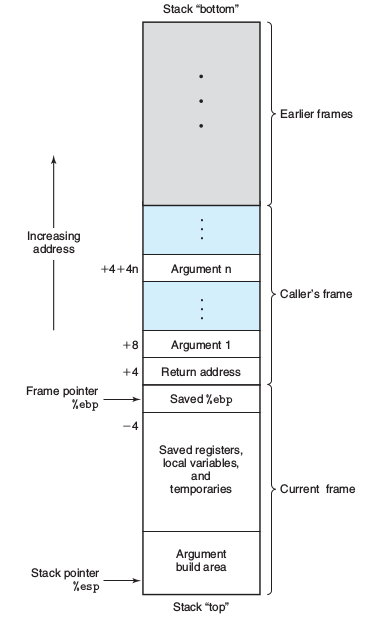
\includegraphics[scale=0.75]{./img/stack2.png}
         \label{img:stack}
         \caption{IA32 Stack Structure}
     \end{figure}

     By convention, certain registers are kept private. Usually the registers {\ttfamily \%eax}, {\ttfamily \%edx}, and {\ttfamily \%ecx} are classified as caller-save registers, that is the registers that are written to by the function caller. On the other hand, the registers {\ttfamily \%ebx}, {\ttfamily \%esi}, and {\ttfamily \%edi} are classified as callee-save registers. That is the registers needed by the called function.

    \subsection{Arrays}
    Arrays are a common tool, and are fairly simplistic in nature. These work in principle by allocating the required memory for the specified data type, and referencing to it in order.

    Structures are treated (to an extent) the exact same as arrays. When a structure is created, the required memory for the data types fills contiguous space in memory.

\newpage
\begin{table}
    \centering
    \begin{tabular}{| p{0.2\textwidth} | l | l | p{0.4\textwidth} |}
        \hline
        Command & Generic Syntax & Example & Description\\
        \hline
        $M[Imm + R[E_b] + R[E_i] \cdot s]$ & $Imm(E_b, E_i, s)$ & {\ttfamily 0xFC(\%eax,\%edx,4)} & Reference memory location based off of preset values.\\
        \hline
        {\ttfamily mov}             & {\ttfamily mov src,dst}    & {\ttfamily mov (\%esp),\%edx}             & Copy the data from the source location to the destination.\\
        {\ttfamily push}            & {\ttfamily push item}      & {\ttfamily push \$0xFF}                   & Push an item onto the stack.\\
        {\ttfamily pop}             & {\ttfamily pop item}       & {\ttfamily pop \$0xFF}                    & Pop an item from the stack.\\
        {\ttfamily leal}            & {\ttfamily leal src,dst}   & {\ttfamily leal 6(\%eax),\%edx}           & Load Effective Address takes whatever {\ttfamily src} points to, and loads it into {\ttfamily dst}.\\
        \hline
        {\ttfamily inc}             & {\ttfamily inc dst}        &                                           & $ dst = dst + 1 $\\
        {\ttfamily dec}             & {\ttfamily dec dst}        &                                           & $ dst = dst - 1 $\\
        {\ttfamily neg}             & {\ttfamily neg dst}        &                                           & $ -dst $\\
        {\ttfamily not}             & {\ttfamily not dst}        &                                           & $ \sim dst $\\
        {\ttfamily add}             & {\ttfamily add src,dst}    &                                           & $ dst = dst + src $\\
        {\ttfamily sub}             & {\ttfamily sub src,dst}    &                                           & $ dst = dst - src $\\
        {\ttfamily imul}            & {\ttfamily imul src,dst}   &                                           & $ dst = dst * src $\\
        {\ttfamily xor}             & {\ttfamily xor src,dst}    &                                           & $ dst = dst \wedge src $\\
        {\ttfamily or}              & {\ttfamily or src,dst}     &                                           & $ dst = dst | src $\\
        {\ttfamily and}             & {\ttfamily and src,dst}    &                                           & $ dst = dst \& src $\\
        {\ttfamily sal}             & {\ttfamily sal k,dst}      &                                           & $ dst = dst << k $\\
        {\ttfamily shl}             & {\ttfamily shl k,dst}      &                                           & $ dst = dst << k$\\
        {\ttfamily sar}             & {\ttfamily sar k,dst}      &                                           & $ dst = dst {>>}_A k $\\
        {\ttfamily shr}             & {\ttfamily shr k,dst}      &                                           & $ dst = dst {>>}_L k $\\
        \hline
        {\ttfamily cmp}             & {\ttfamily cmp src2,src1}  & {\ttfamily cmp \%eax,\%edx}               & Sets flags on {\ttfamily src1 - src2}.\\
        {\ttfamily test}            & {\ttfamily test src2,src1} & {\ttfamily test \%eax,\%edx}              & Sets flags on {\ttfamily src1 \& src2}.\\
        \hline
        {\ttfamily jmp}             & {\ttfamily jmp dst}        &                                           & Direct Jump\\
        {\ttfamily je/jne}          & {\ttfamily jmp dst}        &                                           & Jump equal/not equal\\
        {\ttfamily js/jns}          & {\ttfamily jmp dst}        &                                           & Jump negative/not negative\\
        {\ttfamily jg/jge/jl/jle}   & {\ttfamily jmp dst}        &                                           & Jump greater/less\\
        {\ttfamily ja/jae/jb/jbe}   & {\ttfamily jmp dst}        &                                           & Jump above/below\\
        \hline
        {\ttfamily call}            & {\ttfamily call label}     & {\ttfamily call 8049908}                  & Call procedure for execution\\
        {\ttfamily leave}           & {\ttfamily leave}          &                                           & Prepare stack for return. This sets the stack pointer to the beginning of the frame and restores the saved {\ttfamily \%ebp}.\\
        {\ttfamily ret}             & {\ttfamily ret}            &                                           & Return from call\\
        \hline
    \end{tabular}
    \label{table:assembly}
    \caption{Assembly Reference}
\end{table}

